% !TEX root = paper.tex
\section{Methodology}
\subsection{Tyne and Wear ANPR Data}\label{s.ncl}

\begin{figure}[t]
\centering
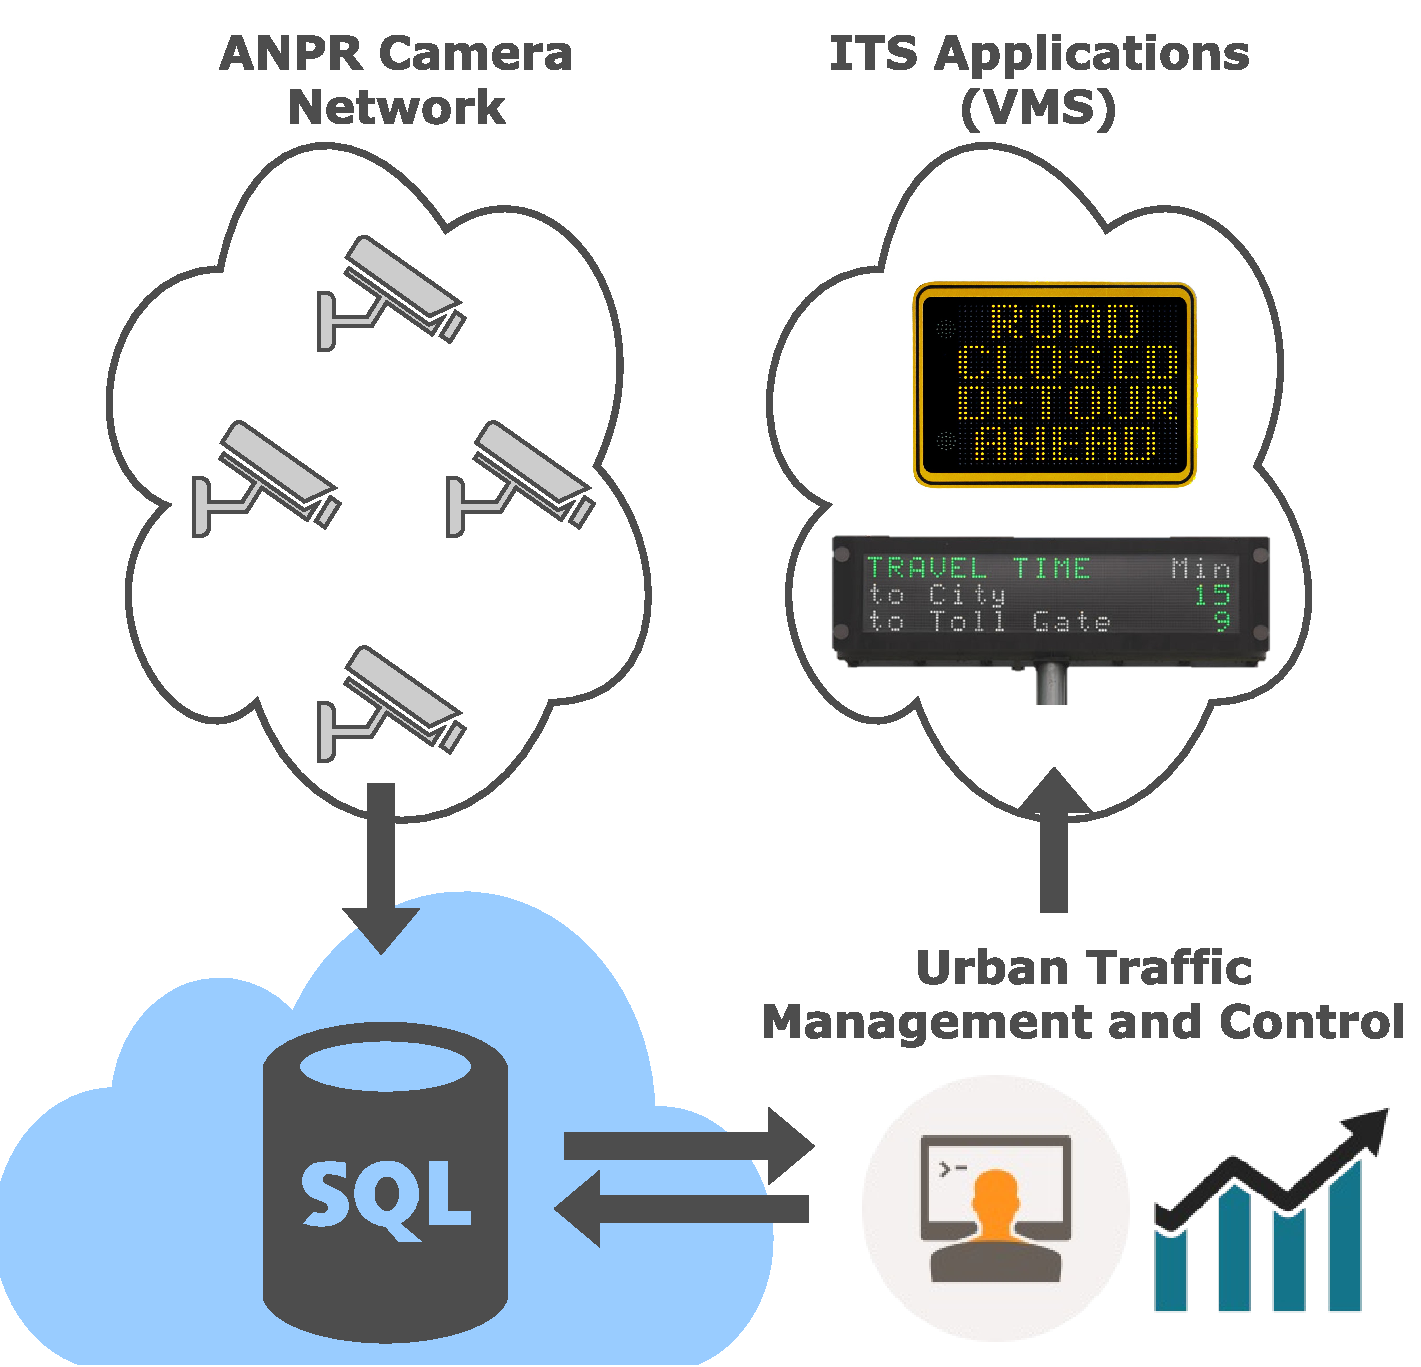
\includegraphics[width=.90\linewidth]{ANPR-overview.pdf}
\caption{Overview of a ANPR-based system for traffic monitoring and control.}
\label{fig:anpr-overview}
\vspace{-0.25cm}
\end{figure}

\begin{figure*}[!ht]
\centering
\begin{subfigure}[t]{.48\textwidth}
  \centering
  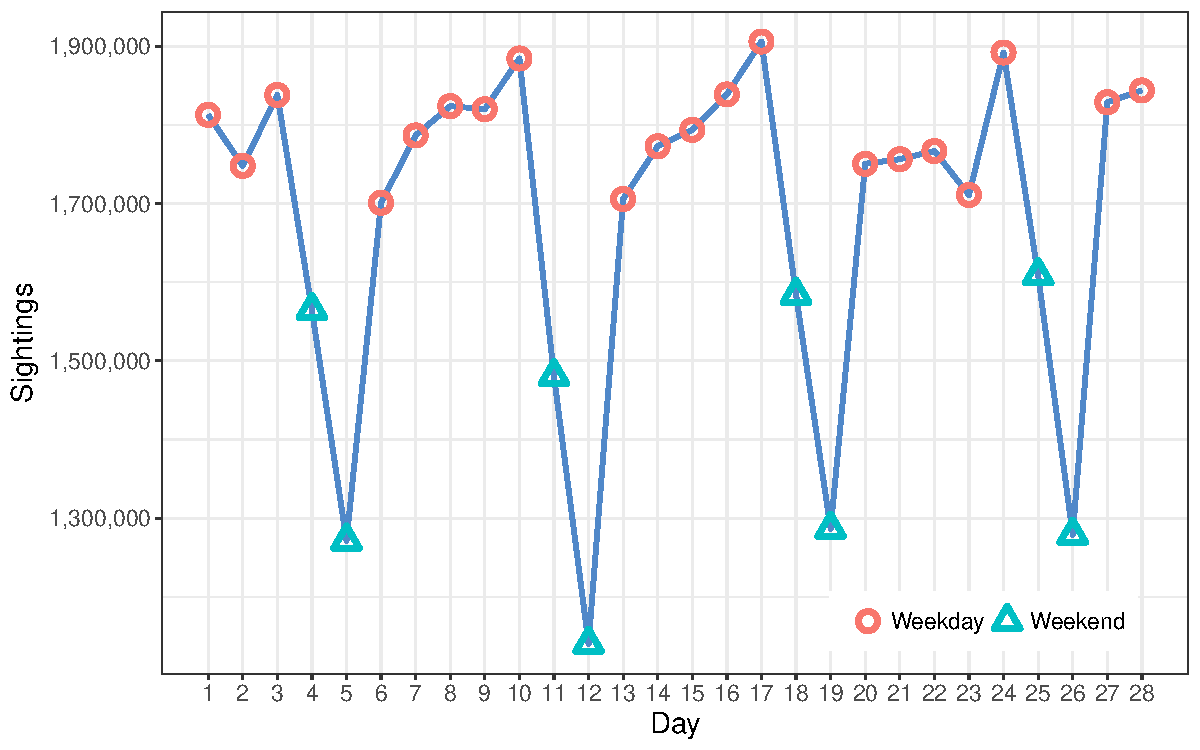
\includegraphics[width=.9\linewidth]{observations_per_day.pdf}
  \caption{Total number of scans recorded per day in Tyne and Wear. There is a clear seasonal effect caused by decreasing traffic demands at weekends and increasing traffic volume during weekdays.}
  \label{fig:observations-per-day}
\end{subfigure}\hfill
\begin{subfigure}[t]{.48\textwidth}
  \centering
  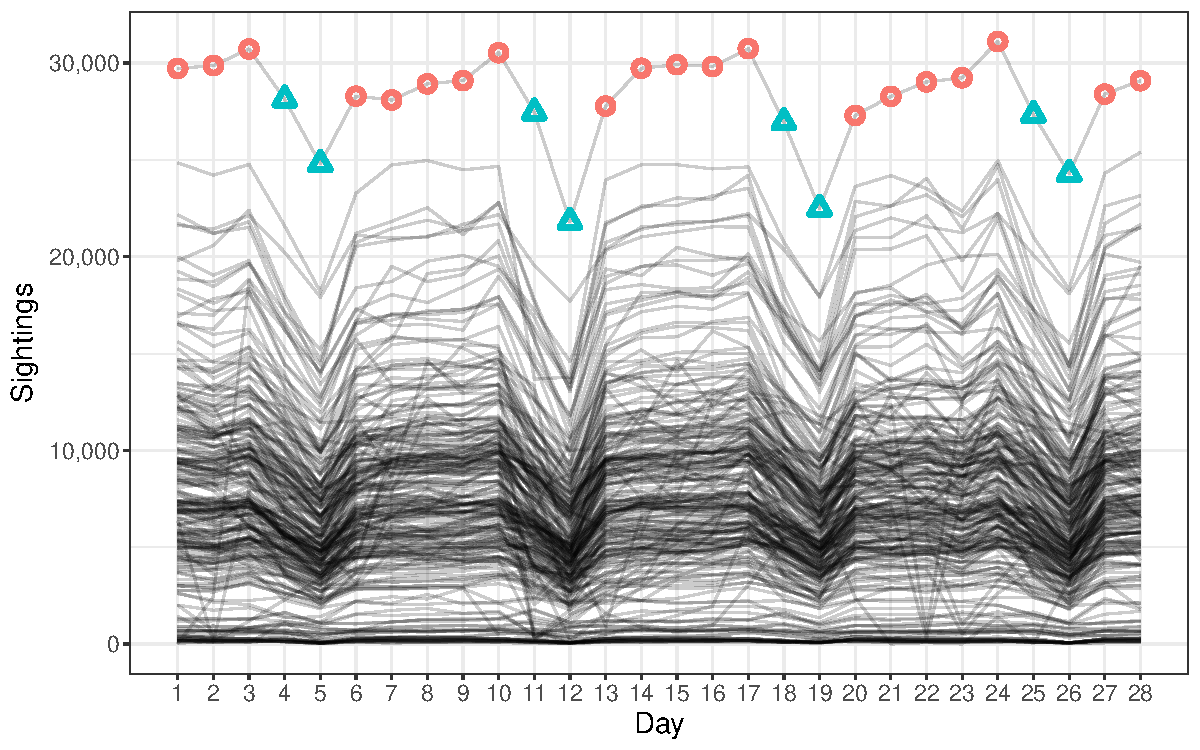
\includegraphics[width=.9\linewidth]{observations_per_day_camera.pdf}
  \caption{Number of scans recorded per ANPR camera and day in Tyne and Wear. Inter-camera variability is observed, as some cameras are located in more traffic intensive road sections than others. Decommissioned or temporarily unavailable cameras (due to loss of power, faulty camera, road closed, etc) can be identified at the bottom.}
  \label{fig:observations-per-camera-day}
\end{subfigure}
\caption{License plate scans recorded by ANPR cameras during February 2017, in the region of Tyne and Wear, United Kingdom.}
\label{fig:time-series}
\vspace{-0.4cm}
\end{figure*}

Automatic num\-ber plate recognition (ANPR) cameras are actively employed in urban traffic environments and play an important role in day-to-day intelligent transportation systems. They can be used by government subsidised entities in urban traffic management and control; by commissioned highway agencies in electronic toll collection; or by law enforcement organisations in detecting speeding vehicles and validating number plate registrations. The wide diversity of applications, paired with the large improvements in price-to-performance ratios of ANPR hardware and software systems, has resulted in increased investments of ANPR cameras for urban environments~\cite{EvolutionUTMC2013, SurveyITS2011}.

In the region of Tyne and Wear, United Kingdom, there are over 250 active ANPR cameras. Over 1 million license plate detections are recorded by these cameras every day. Figure~\ref{fig:time-series} shows the number of daily scans recorded over a month (February, 2017). Furthermore, every scan is stored in a central database managed by the Tyne and Wear UTMC, and used to compute travel times across particular links of interest in the road network. These are usually major roads that see high volumes of traffic, or road segments more prone to traffic jams. Average journey times can then be conveyed back to the drivers by the way of Variable Message Signs (VMS) or web based applications. Figure~\ref{fig:anpr-overview} represents this interaction.

Number plate data, in its essence, is a stream of events, each representing a vehicle observed by one camera at a specific point in time. An excerpt of the data can be found in Table~\ref{t:np_data_example}. All number plate were anonymised by the UTMC through a hashing algorithm before the data was shared. Cameras are uniquely identified by an integer and timestamps are relative to each camera's clock. Clock synchronisation is performed using the Network Time Protocol (NTP), as the cameras are connected, through a private network, to a central server. Therefore, the recorded timestamps can be used directly if the synchronisation error is negligible. The following additional information is also captured and provided by each camera:
\begin{enumerate*}[label=(\roman*)]
  \item the clock synchronisation error (milliseconds);
  \item the camera's confidence that the identified number plate is the true number plate (percentage);
  \item the direction of travel, away or towards the camera.
\end{enumerate*}
The confidence in the observation is especially useful as it helps diagnosing license plate recognition errors. On the other hand, the direction of travel is dependent upon the orientation of the camera, which is not provided. Hence, we chose to ignore the latter in this work.

\begin{table}[t]
\centering
\tabcolsep=0.12cm
\begin{tabular}{c c c c c}
  \hline
  Vehicle & Camera & Timestamp & \thead{Clock \\Error} & Confidence \\
  \hline
  169239 & 1031 & 1454284800.26 &   0 & 100 \\
  12862943 & 18 & 1454284800.97 &   8 &  61 \\
  16243894 & 22 & 1454284801.46 &   6 &  86 \\
  4817789 & 52 & 1454284803.43 &  13 &  94 \\
  5503486 & 110 & 1454284802.19 &  22 &  91 \\
  15244177 & 115 & 1454284802.83 &  18 &  87 \\
   \hline
\end{tabular}
\caption{Sample of number plate data. Clock error is given in milliseconds and confidence as a percentile value.}
\label{t:np_data_example}
\vspace{-0.3cm}
\end{table}
